%\customlink{magnetic_mineralogy}%Lori don't change this
\chapter{Magnetic mineralogy}


\noindent
BACKGROUND: Evans and Heller (2003), Chapter 3.  \nocite{evans03}
\vskip 24pt

An essential part of every paleomagnetic study is a discussion of what is
carrying the magnetic remanence and how the rocks got magnetized.  For this, we
need some knowledge of what the important natural magnetic phases are, how to
identify them,  how they formed, and what their magnetic behavior is. 
In this chapter, we will  cover a brief description of geologically important magnetic
phases. Useful magnetic characteristics of important minerals
can be found in Table~\ref{tab:rockpars} at the end of this chapter.

Iron is by far the most abundant transition element in the solar system, so most
paleomagnetic studies depend on the magnetic iron bearing minerals: the iron-nickels
(which are particularly important for extra-terrestrial magnetic studies), the 
iron-oxides such as magnetite, maghemite  and hematite, the  iron-oxyhydroxides such as goethite and ferrihydrite, and the iron-sulfides such as greigite and pyrrhotite. 
 We are concerned here with the latter three as iron-nickel is very rare in terrestrial paleomagnetic studies.  

 
 
 \section {Iron-oxides}
 
 The minerals we will be discussing are mostly
 \index{solid solutions}
{\it solid solutions} which the American Heritage dictionary defines  as:
 
 \begin{quote}
A homogeneous crystalline structure in which one or more types of atoms or molecules may be partly substituted for the original atoms and molecules without changing the structure.
\end{quote}

In  iron oxides, titanium commonly substitutes for iron in the crystal structure.  Because the titanium ion Ti$^{4+}$ has no unpaired spins (see Chapter 3) and is a different size, the magnetic properties of titano-magnetite are different from magnetite with no titanium.   




 Two solid solution series are particularly important in paleomagnetism: the
 \index{ulv\"ospinel}
 \index{magnetite}
 \index{ilmenite}
 \index{hematite}
 \index{titanomagnetite}
 \index{hemoilmenite}
ulv\" ospinel-magnetite and ilmenite-hematite series.    Both titanomagnetites and hemoilmenites crystallize at about 1300$^{\circ}$C.   
 Above about 600$^{\circ}$C, there is complete solid solution between magnetite and ulv\"ospinel and above about 800$^{\circ}$C between hematite and ilmenite.   This means that all compositions are ``allowed'' in the crystal structure at the crystallization temperature.  As the temperature decreases, the thermodynamic stability of the crystals changes.   If a mineral has a given composition, say 60\% titanium substitution (green dot in Figure~\ref{fig:solidsolution}a), when the temperature cools to intersect the red line, that composition is no longer thermodynamically stable and the two phases to either side are the equilibrium compositions.   By 400$^{\circ}$C the two equilibrium phases are $\sim$0.25 and $\sim$0.9 Ti substitution.   To achieve the separation, the  cations diffuse through the crystal leaving titanium richer and titanium poorer bands called {\it lamellae}  (see Figure~\ref{fig:exsolution}).   Exsolution is inhibited if the crystals cool rapidly so there are many metastable crystals with non-equilibrium values of titanium substitution in nature.
 
\begin{figure}[htb]
%\epsfxsize 13cm
%\centering \epsffile{EPSfiles/solidsolution.eps}
\centering  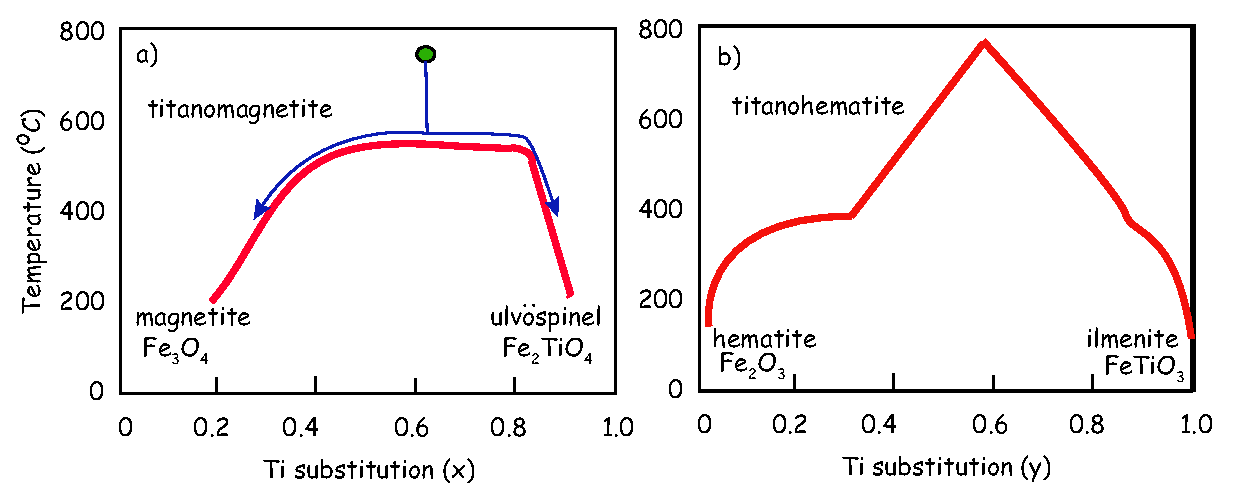
\includegraphics[width=13 cm]{EPSfiles/solidsolution.eps}
\caption{Phase diagrams for FeTi oxides.  The composition is indicated by $x$ or $y$. 
There is complete solid solution above the solid lines.  Exolution begins as the temperature cools below the solid curves.  a) Titanomagnetite series. [Redrawn from Nagata, 1961.] b) Titanohematite series.  [Redrawn from Robinson et al. 2004.]}
\label{fig:solidsolution}
\end{figure}
 \nocite{robinson04} \nocite{nagata61}


\index{exsolution} 
 Exsolution is important in paleomagnetism for two reasons.  First, the different compositions have very different magnetic properties.  Second,  the lamellae effectively reduce the magnetic crystal size which we already know has a profound influence on the magnetic stability of the mineral.   An example of this is shown in Figure~\ref{fig:exsolution}b in which the larger crystal is  several microns in width, too large to have single domain-like magnetization, yet the smaller magnetite lamellae are indeed small enough and carry a strong stable magnetization 
 \index{Feinberg, J.M.}
 (Feinberg et al. 2005). \nocite{feinberg05}


\begin{figure}[htb]
%\epsfxsize 12cm
%\centering \epsffile{EPSfiles/exsolution.eps}
\centering  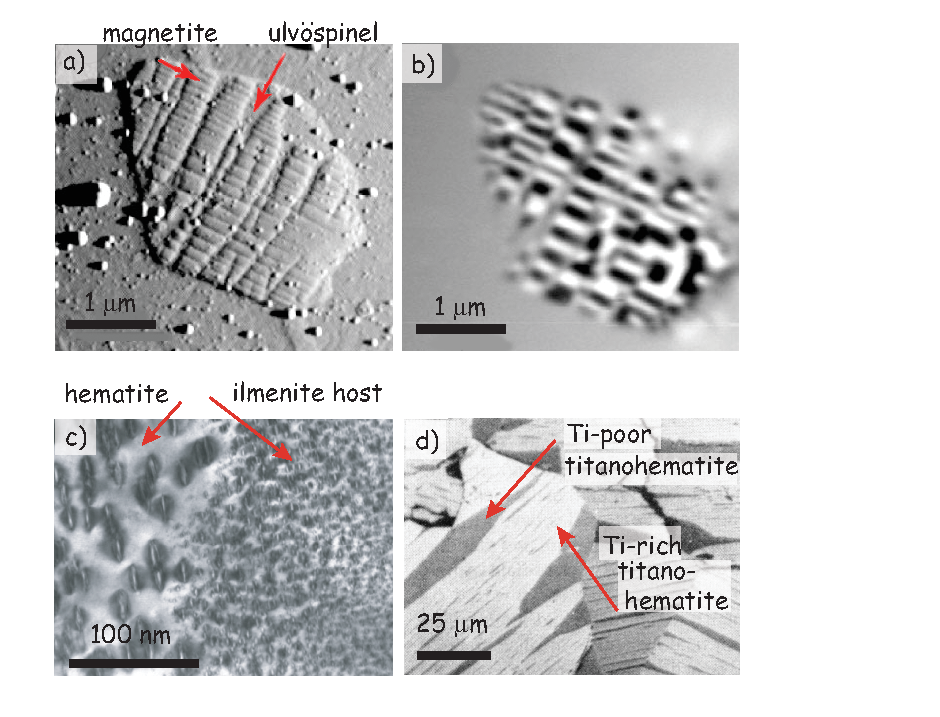
\includegraphics[width=12 cm]{EPSfiles/exsolution.eps}
\caption{a) Atomic force micrograph image of magnetite inclusion in clinopyroxene.  The topographically low areas are ulv\"ospinel while the higher areas are magnetite.  b) Magnetic force micrograph of magnetic domains (black and white are oppositely magnetized).  The ulv\"ospinel lamellae are essentially non-magnetic and are gray    c) Tranmission electron micrograph of ilmenite host with hematite exolution lamellae.  Lamellar size gets smaller  with proximity to edge.   d) Photomicrograph of  titanohematite exolution lamellae. Dark bands are Ti-rich (high  magnetization, low $T_c$), light grey bands are Ti-poor (low magnetization, high $T_c$).  [a and b are from Feinberg et al., 2005, c) from Robinson et al., 2002., d) is modified from S. Haggerty in Butler (1992).]}
\label{fig:exsolution}
\end{figure}
\nocite{feinberg05,robinson02,butler92}

 
 
\begin{figure}[htb]
%\epsfysize 3in
 %\centering \epsffile {EPSfiles/tern.eps}
\centering  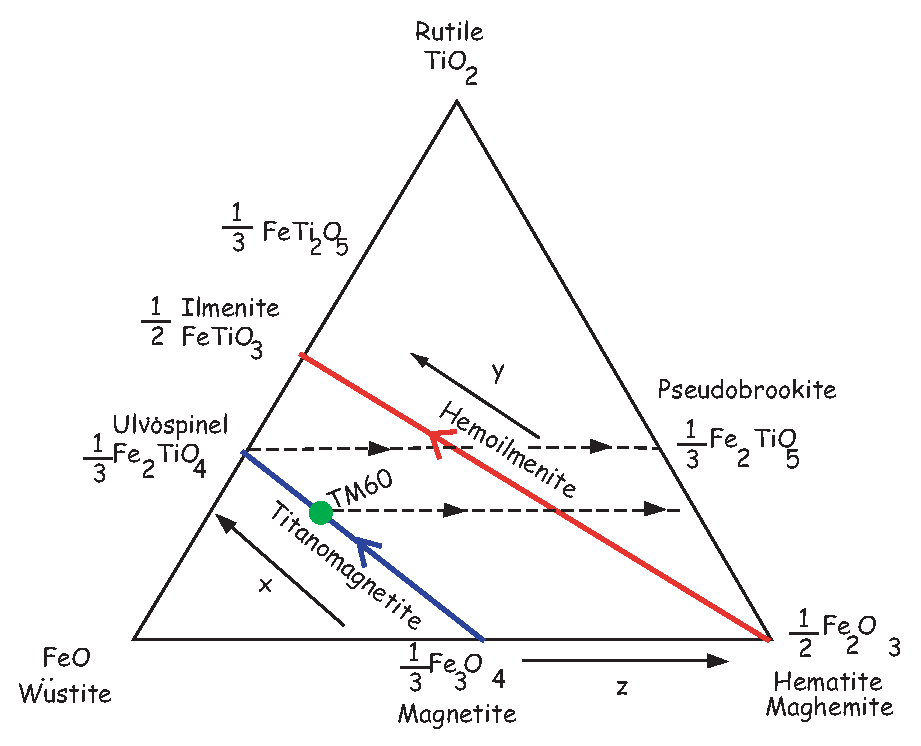
\includegraphics[width=3 in]{EPSfiles/tern.eps}
\caption{Ternary diagram for iron-oxides.
The solid lines are solid solution series with increasing titanium concentration ($x$). 
The dashed lines with arrows indicate the direction of increasing
oxidation ($z$). [Figure redrawn from  Butler, 1992.] }
\label{fig:tern}
\end{figure}
 \nocite{oreilly84}

Compositions of minerals are frequently plotted on 
\index{diagrams!ernary}
ternary diagrams like the one shown in Figure~\ref{fig:tern}.  [For help in reading ternary diagrams, please see the Appendix~\ref{app:ternary}]  
The apices of the ternary diagram are Fe$^{2+}$ on the lower left, Fe$^{3+}$ on the lower right and Ti$^{4+}$ on the top.   The oxides with these species are FeO (w\"ustite),  Fe$_2$O$_3$ (hematite or maghemite depending on structure) and TiO (rutile).  Every point on the triangle represents a cation mixture or solution that adds up to one cation (hence the fractional formulae).  

Each of the solid arrows in Figure~\ref{fig:tern} (labelled titanomagnetite and hemoilmenite) represent
increasing substitution of titanium into the crystal lattices of magnetite and
hematite respectively.
  The amount of Ti substitution in
titanomagnetites is denoted by ``$x$'', while substitution in the
hemoilmenites is denoted by ``y''.
Values for $x$ and $y$  range from 0 (magnetite or hematite) to 1 
(ulv\"ospinel or ilmenite).    






\subsection {Titanomagnetites Fe$_{3-x}$Ti$_x$O$_4$} 
\label{sect:titano}

\index{magnetite}%
\index{inverse spinel}%
\index{titanomagnetite}
In earlier chapters on rock magnetism, we learned a few things about magnetite.  As mentioned in Chapter 4, magnetite (Fe$_3$O$_4$) has an
inverse spinel structure (AB$_2$O$_4$).  The oxygen atoms form a face-centered cubic
lattice into which cations fit in either octahedral or tetrahedral symmetry. 
 For each
unit cell there are four tetrahedral sites (A) and eight octahedral sites (B). 
To maintain charge balance with the four oxygen ions (O$^{2-}$), 
there are two Fe$^{3+}$ ions
and one Fe$^{2+}$ ion. 
Fe$^{3+}$ has five unpaired spins, while Fe$^{2+}$ has four.  As
discussed in Chapter  3, each unpaired spin contributes a moment of one 
\index{Bohr magneton}% 
Bohr magneton ($m_b$). 
The divalent iron ions all reside in the octahedral lattice
sites, whereas  the trivalent iron ions are split evenly between octahedral and
tetrahedral sites: Fe$^{3+}|$Fe$^{3+}$Fe$^{2+}|$O$_4$.  The A and B lattice sites are
coupled with antiparallel spins and magnetite is ferrimagnetic.
Therefore, the net moment of  magnetite is (9-5=4)  $m_b $ per molecule
(at 0 K).

 \begin{figure}[htb]
%\epsfxsize 14cm
%\centering \epsffile{EPSfiles/X.eps}
\centering  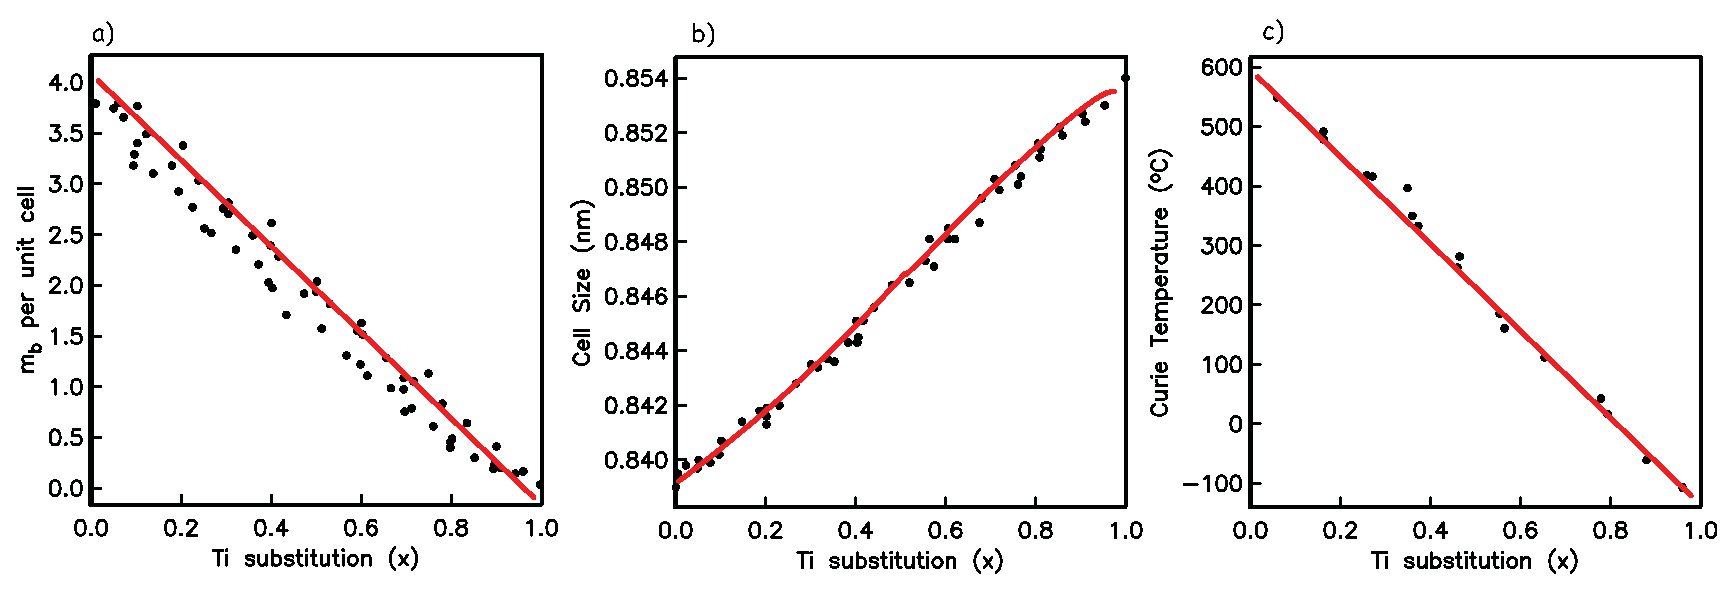
\includegraphics[width=14 cm]{EPSfiles/X.eps}
\caption{Variation of intrinsic parameters with titanium substitution in the titanomagnetite lattice.  X is the degree of substitution from 0 (no Ti) to 1 (100\% substitution).  a) Variation of the magnetization expressed as Bohr magnetons per unit cell.  b) Variation of cell lattice size.  c) Variation of Curie temperature. [Data compiled by O'Reilly, 1984.])}
\label{fig:X}
\end{figure} \nocite{oreilly84}


Titanomagnetites can occur 
as  primary minerals in igneous rocks.  Magnetite, as well as various
members of the hemoilmenite series, can also form as a
result of high temperature 
oxidation.  In sediments, magnetite often occurs as a 
detrital component.  It can
also be produced by bacteria or authigenically during diagenesis.

Substitution of Ti$^{4+}$, which has no unpaired spins (see Chapter 3),
 has a profound effect on the magnetic properties of the
resulting titanomagnetite.  Ti$^{4+}$ substitutes for a trivalent iron ion.
In order to maintain charge balance, another trivalent iron ion turns into a divalent iron
ion.  The end members of the solid solution series are:

\begin{center}
\begin{tabular}{cc}
\hline
 magnetite  &  ulv\"ospinel \\
 Fe$^{3+}|$Fe$^{3+}$Fe$^{2+}|$O$_4$  &  Fe$^{2+}|$Fe$^{2+}$Ti$^{4+}|$O$_4$ \\
 $x = 0 $ &  $x=1$  \\
\hline
\end{tabular}
\end{center}

\begin{figure}[htb]
%\epsfxsize 14cm
%\centering \epsffile{EPSfiles/hematite.eps}
\centering  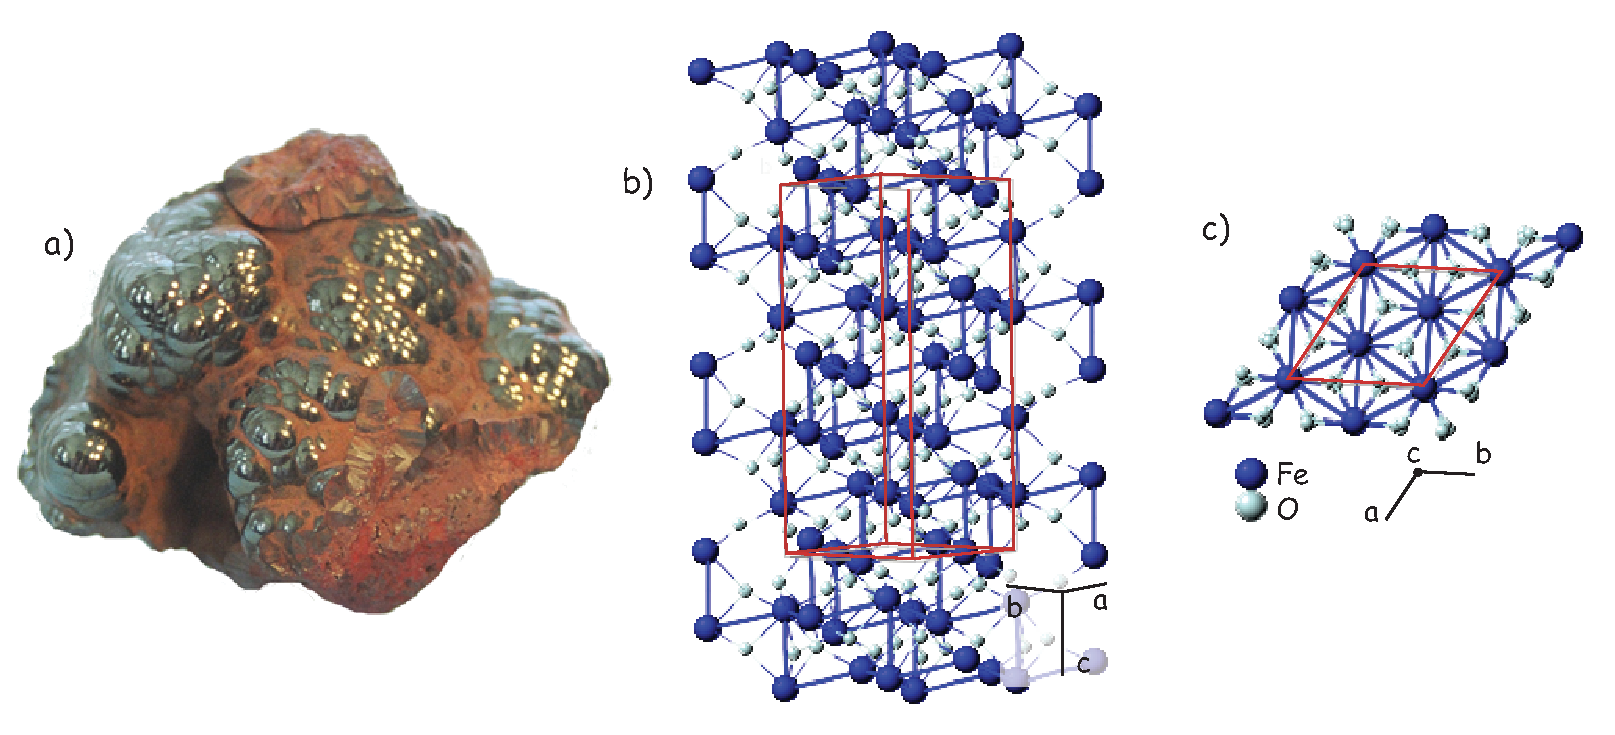
\includegraphics[width=14 cm]{EPSfiles/hematite.eps}
\caption{Hematite. a) Photograph of Kidney ore hematite from Michigan by DanielCD. [From commons.wikimedia.org/wiki/File:Hematite.jpg.]   b-c) Two views of the crystal structure of hematite.  c-axis is perpendicular to the basal plane. [From \href{http://www.webmineral.com}{http://www.webmineral.com}.] }
\label{fig:hematite}
\end{figure} 


\index{antiferromagnetism}%
\index{ulv\"ospinel}%
Ulv\" ospinel is antiferromagnetic because the A and B lattice sites have the
same net moment.  When $x$ is between 0 and 1, the mineral is called a
titanomagnetite.  If $x$ is 0.6,  for example, the mineral
is called TM60 (green dot in Figure~\ref{fig:tern}).  

\index{titanium substitution}%
The profound effect of titanium substitution on the intrinsic properties of titanomagnetite is illustrated in Figure~\ref{fig:X}.  Because Ti$^{4+}$ has no unpaired spins, the saturation magnetization decreases with increasing $x$ (Figure~\ref{fig:X}a).   The cell dimensions increase with increasing $x$ (Figure~\ref{fig:X}b).  As a result of the increased cell dimension, there is a decrease in
\index{Curie temperature}
 Curie Temperature (Figure~\ref{fig:X}c).  There is also a    slight increase in  coercivity (not shown).  

The large $M_s$ of magnetite (see Table~\ref{tab:rockpars}) means that
for deviations from equant grains as small as 10\%, 
\index{magnetic!anisotropy energy}%
the magnetic anisotropy energy becomes dominated by shape. 
Nonetheless, aspects of the
\index{magnetic!anisotropy!energy!magnetocrystalline}%
magnetocrystalline anisotropy provide useful diagnostic tests.  The
magnetocrystalline anisotropy constants are a strong function of
temperature. On warming to $\sim$-100$^{\circ}$C from
near absolute zero, changes in
these constants can lead to an abrupt loss of magnetization, which is
known loosely as the 
\index{Verwey transition}%
{\it Verwey transition} (see Chapter 4).  Identification of the Verwey
transition suggests a remanence that is dominated by magnetocrystalline
anisotropy.  As we shall see, 
the temperature at which it occurs is sensitive to oxidation and the
transition can be
completely supressed by maghemitization (see 
Dunlop and \"Ozdemir [1997]). 

It should be noted that natural titanomagnetites often contain impurities (usually Al, Mg, Cr).  These impurities also affect the magnetic properties.   Substitution of 0.1 Al$^{3+}$ into the unit cell of titanomagnetite results in a 25\% reduction in $M_s$ and a reduction of the Curie temperature by some 50$^{\circ}$C.  Substitution of Mg$^{2+}$ into TM60 also results in a lower saturation magnetization with a reduction of some 15\%. 

\begin{figure}
%\epsfxsize 14cm
%\centering \epsffile{EPSfiles/hemY.eps}
\centering  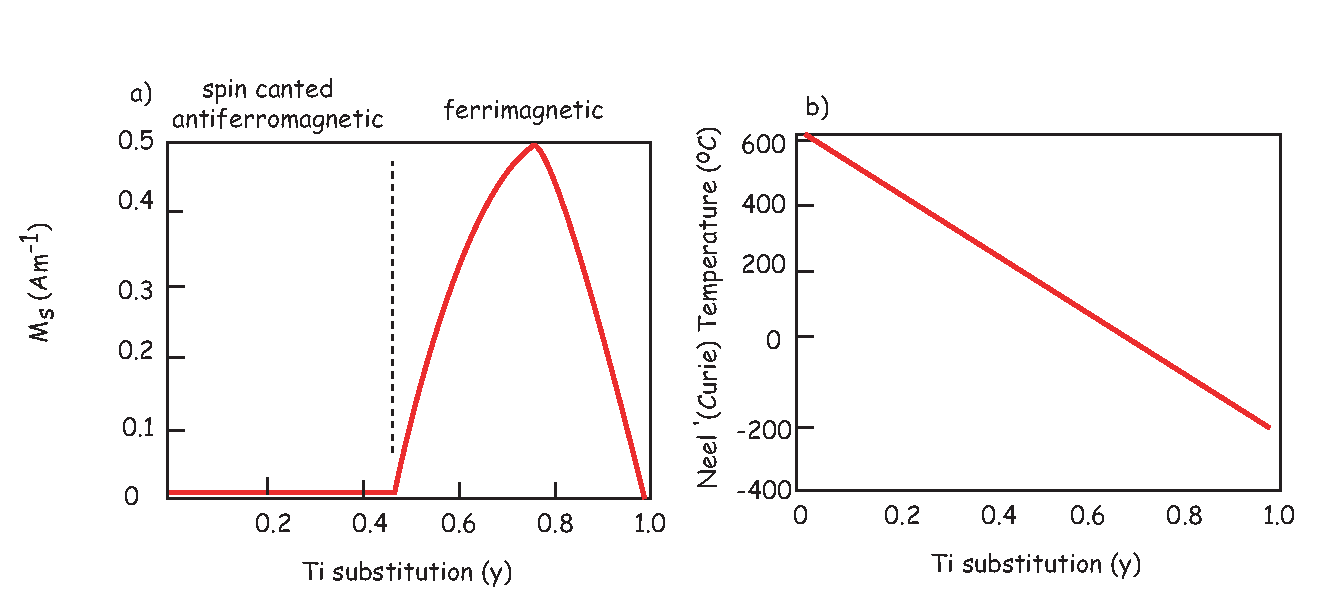
\includegraphics[width=14 cm]{EPSfiles/hemY.eps}
\caption{Variation of properties with Ti substitution in the titanohematite series.  a) Variation of saturation magnetization.  b) Variation of N\'eel Temperature.  [Modified from Nagata, 1961 and Stacey and Banerjee, 1974.]}
\label{fig:hemY}
\end{figure}
\nocite{nagata61,stacey74}



\subsection {Hematite-Ilmenite Fe$_{2-y}$Ti$_y$O$_3$}
\label{sect:hemo}

\index{hematite}%
Hematite has a corundum  structure (see Figure~\ref{fig:hematite}).  It is rhombohedral with a pseudocleavage
(perpendicular to the $c$ axis) and  tends to break into flakes.  
It is
antiferromagnetic, with a weak 
parasitic ferromagnetism  resulting from either 
spin-canting or 
defect ferromagnetism (see Chapter 3).
 Because the magnetization is a spin canted antiferromagnetism, the temperature at which this magnetization disappears is called the 
 \index{N\'eel!temperature}
 N\'eel Temperature instead of the Curie Temperature which is {\it sensu strictu} only for ferromagnetic minerals.  
The N\'eel temperature for hematite is approximately 685$^{\circ}$C.  


  Above about -10$^{\circ}$C (the 
\index{Morin transition}%
{\it Morin
transition}), the magnetization is constrained by aspects of the crystal
structure to lie
perpendicular to the $c$ axis or within the basal plane.  Below the Morin transition, 
\index{spin-canting}
spin-canting all but disappears
and the magnetization is parallel to the $c$ axis.  This effect could be used to
demagnetize the grains dominated by spin-canting: it 
does not affect those dominated by defect
moments.   Most hematites  formed at  low-temperatures have magnetizations dominated by defect moments, so the remanence of many rocks will not display a Morin transition.


 \begin{figure}[h!tb]
%\epsfxsize 14cm
%\centering \epsffile{EPSfiles/Z.eps}
\centering  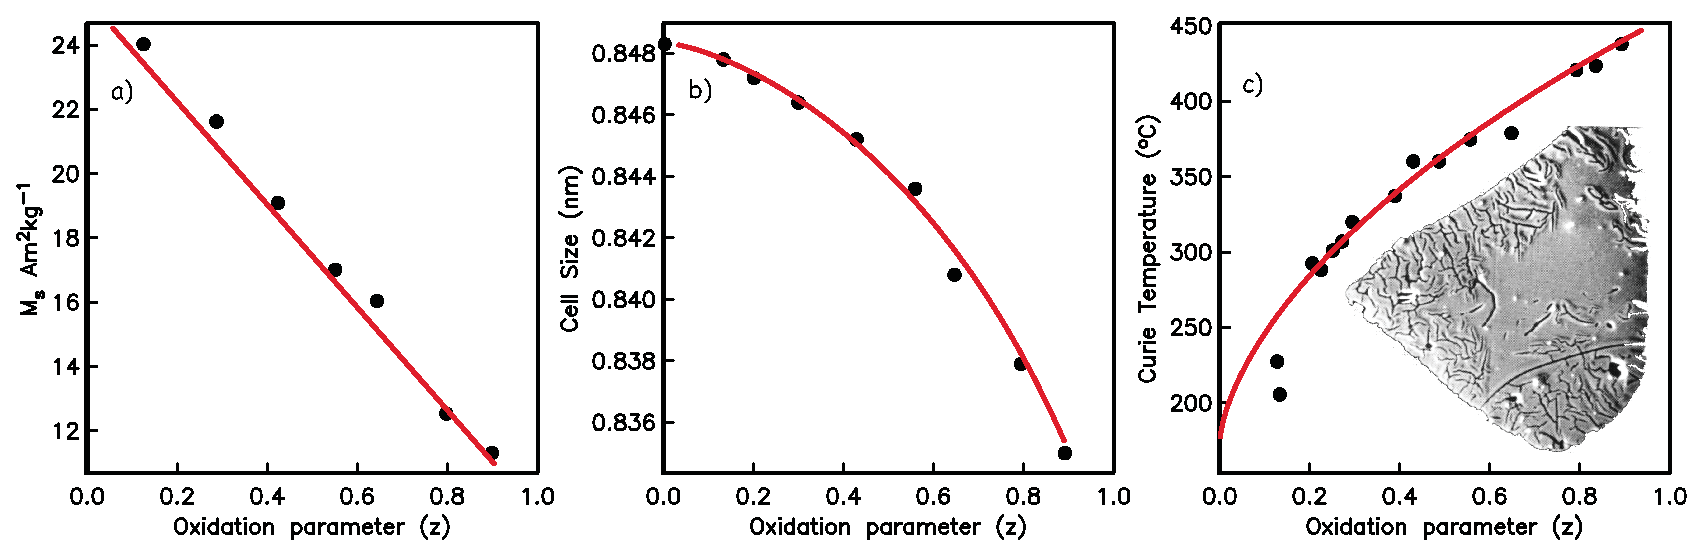
\includegraphics[width=14 cm]{EPSfiles/Z.eps}
\caption{Variation of intrinsic parameters with oxidation in TM60.  $z$ is the degree of oxidation.  a) Variation of the magnetization.   b) Variation of cell lattice size.  c) Variation of Curie temperature. [Data compiled by Dunlop and \"Ozdemir, 1997.]  inset: A magnetite crystal ($\sim$ 30 $\mu$m) undergoing maghemitization.  Because of the change in volume, the crystal begins to crack. [From Gapeyev and Tsel'movich, 1988 in Dunlop and \"Ozdemir, 1997.]}
\label{fig:Z}
\end{figure}\nocite{gapeyev88}


Hematite occurs widely in oxidized sediments and dominates the magnetic
properties of red beds.  It occurs as a high temperature oxidation product 
in certain igneous rocks.  Depending on grain size, among
other things, it is either
black (specularite) or red (pigmentary).  Diagnostic properties of hematite are listed in Table~\ref{tab:rockpars}.



The substitution of Ti into the lattice structure of $\alpha$Fe$_2$O$_3$ has an even more profound influence on magnetic properties  than for magnetite.  For $y=0$ the magnetization is spin-canted antiferromagnetic, but when $y=0.45$, the magnetization becomes ferrimagnetic (see Figure~\ref{fig:hemY}a).   For small amounts of substitution, the Ti and Fe cations are distributed equally among the cation layers.  For $y>0.45$, however, the Ti cations preferentially occupy alternate cation layers.  Remembering that the Ti$^{4+}$  ions have no net moment, we can imagine  that antiparallel coupling between the two sub-lattices results in ferrimagnetic behavior, as opposed to the equal and opposite style of anti-ferromagnetism.  



\index{titanohematite}
Titanohematite particles with intermediate values of $y$ have interesting properties from a paleomagnetic point of view.   There is a solid solution at high temperatures, but as the temperatures drop the crystals exsolve into titanium rich  and poor  lamellae (see Figure~\ref{fig:exsolution}d).  Figure~\ref{fig:hemY} shows the variation in saturation magnetization and N\'eel  temperature with Ti substitution.   For certain initial liquid compositions, the exolution lamellae could have Ti-rich bands alternating with Ti-poor bands.  If the Ti-rich bands have higher magnetizations, yet lower Curie temperatures than the Ti-poor bands, the Ti-poor bands will become magnetized first.  When the Curie temperature of the Ti-rich bands is reached, they will become magnetized in the presence of the demagnetizing field of the Ti-poor bands, hence they will acquire a remanence that is antiparallel to the applied field.  Because these bands have higher magnetizations, the net NRM will also be anti-parallel to the applied field and the rock will be {\it self-reversed}.   This is fortunately very rare in nature.


 \begin{figure}[htb]
%\epsfxsize 11cm
%\centering \epsffile{EPSfiles/suppress.eps}
\centering  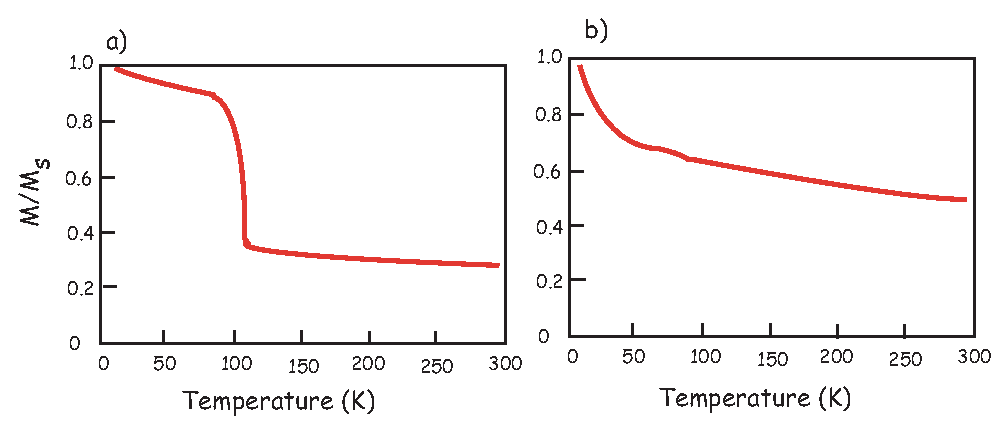
\includegraphics[width=11 cm]{EPSfiles/suppress.eps}
\caption{Effect of maghemitization on Verwey transition.  a) Saturation remanence acquired at 10 K observed as it warms up for 37 nm stoichiometric magnetite.  b) Same but for partially oxidized magnetite. [Data from \"Ozdemir et al., 1993.]  }
\label{fig:suppress}
\end{figure}
\nocite{ozdemir93}


\subsection {Oxidation of (titano)magnetites to (titano)maghemites}

Many minerals form under one set of equilibrium conditions (say within a cooling lava flow) and are later subjected to a different set of conditions (sea-floor alteration or surface weathering).  They will tend to alter in order to come into equilibrium with the new set of conditions.   The new conditions are often more oxidizing than the original conditions and compositions tend to move along the dashed lines in Figure~\ref{fig:tern}.    The degree of oxidation is represented by the parameter $z$. 

While the solid solution between magnetite and ulv\"ospinel exists in principle, intergrowths of these two minerals are actually quite rare in nature because the titanomagnetites interact with oxygen in the melt to form intergrowths of low Ti magnetite with ilmenite.  This form of oxidation is known as 
\index{deuteric oxidation}
{\it deuteric} oxidation.  


 

Low temperature oxidation will tend to transform a single phase spinel (titanomagnetite) into a new single phase spinel (titanomaghemite) by diffusion of  Fe$^{2+}$ from the lattice structure of the (titano)magnetite to the surface where it is converted to Fe$^{3+}$;  
\index{titanomaghemite}
titanomaghemite   is a ``cation-deficient''  inverse  spinel.     The inset to  Figure~\ref{fig:Z}c shows a magnetite crystal in the process of becoming maghemite.  The conversion of the Fe$^{2+}$ ion means a loss in volume which results in characteristic cracking of the surface.   There is also a loss in magnetization, a shrinkage of cell size and, along with the tightening unit cell, an increase in Curie Temperature.  These trends are shown for TM60 in Figure~\ref{fig:Z}.  Maghematization results in a much reduced Verwey transition (see Figure~\ref{fig:suppress}).  


 


 The (titano)maghemite  structure is metastable and can invert to form the isochemical, but more stable structure of (titano)hematite, or it can be reduced to form magnetite.    The two forms of Fe$_2$O$_3$ are distinguished by the symbols $\gamma$ for maghemite and $\alpha$ for hematite.    Inversion of natural maghemite is usually complete by about 350$^{\circ}$C,
but it can survive until much higher temperatures (for more details, see
\index{Dunlop, D.J.}
\index{\"Ozdemir, \"O.}
\nocite{dunlop97}
 Dunlop and \"Ozdemir, 1997).     Also, it is common that the outer rim of the magnetite will be oxidized to maghemite, while the inner core remains magnetite.    


 
\begin{figure}[htb]
%\epsfxsize 14cm
%\centering \epsffile{EPSfiles/minerals.eps}
\centering  \includegraphics[width=14 cm]{EPSfiles/minerals.eps}
\caption{  a) Photograph of goethite. [From  en.wikipedia.org/wiki/Image:Goethite3.jpg; photo of  Eurico Zimbres.]   b) Goethite crystal structure. 
c) Photograph of greigite.  [Photo of William P\'eraud.]   d) Greigite crystal structure. 
e) Photograph of single crystal of pyrrhotite. [Photo of Dan Weinrich.]  f) Pyrrhotite crystal structure.  [All crystal structure images from \href{http://www.webminerals.com}{http://www.webminerals.com}.]}
\label{fig:minerals}
\end{figure}


\section {Iron-oxyhydroxides and iron-sulfides}
\label{sect:pyrrho}

\index{iron-oxyhydroxides}%
Of the many  iron oxyhydroxides that occur in any abundance
in nature, 
\index{goethite}%
goethite ($\alpha$FeOOH; Figure~\ref{fig:minerals}a,b) is the most common magnetic phase. It is
\index{antiferromagnetism}%
\index{defect ferromagnetism}%
antiferromagnetic with what is 
most likely a defect magnetization.  It occurs
widely as a weathering product of iron-bearing minerals and as a direct
precipitate from iron-bearing solutions.  It is metastable  under
many conditions and dehydrates to
hematite with time or elevated temperature.  Dehydration is usually complete by
about 325$^{\circ}$C.  It is characterized by a very high coercivity but a low 
\index{N\'eel!temperature}
N\'eel
temperature of about 100--150$^{\circ}$C.
 Diagnostic properties of goethite are listed in Table~\ref{tab:rockpars}.
 


There are two 
\index{iron-sulfides}%
iron-sulfides that are important to paleomagnetism: 
\index{greigite}%
greigite (Fe$_3$S$_4$; Figure~\ref{fig:minerals}c,d) and
\index{pyrrhotite}%
pyrrhotite (Fe$_7$S$_8$-Fe$_{11}$S$_{12}$; Figure~\ref{fig:minerals}e,f).  These are ferrimagnetic and occur in reducing environments.  They 
both  tend to oxidize to various iron oxides leaving paramagnetic 
\index{pyrite}%
pyrite as the
sulfide component.  


The Curie temperature of 
\index{pyrrhotite!monoclinic}
monoclinic pyrrhotite (Fe$_7$S$_8$)
is about 325$^{\circ}$C (see Figure~\ref{fig:pyrrhotiteT}b; Table~\ref{tab:rockpars}). Monoclinic pyrrhotite undergoes a transition 
at $\sim$ 35 K, so low temperature measurements can be diagnostic for this phase (see Figure~\ref{fig:pyrrhotiteT}a).   
\index{pyrrhotite!hexagonal}
Hexagonal pyrrhotite undergoes a structural transition from an imperfect antiferromagnet to a ferromagnet with much higher saturation magnetization at about 200$^{\circ}$C.  During a thermomagnetic experiment, the expansion of the crystal results in a large peak  in magnetization just below the Curie Temperature (see Figure~\ref{fig:pyrrhotiteT}c).    Mixtures of monoclinic and hexagonal pyrrhotite result in the behavior sketched in Figure~\ref{fig:pyrrhotiteT}d.   
The maximum unblocking temperature of
\index{greigite}
 greigite is approximately
330$^{\circ}$C. 
 Other diagnostic properties of greigite and pyrrhotite are listed in 
Table~\ref{tab:rockpars}.




\begin{figure}[htb]
\centering
%\epsfxsize 14cm
% \epsffile{EPSfiles/pyrrhotiteT.eps}
 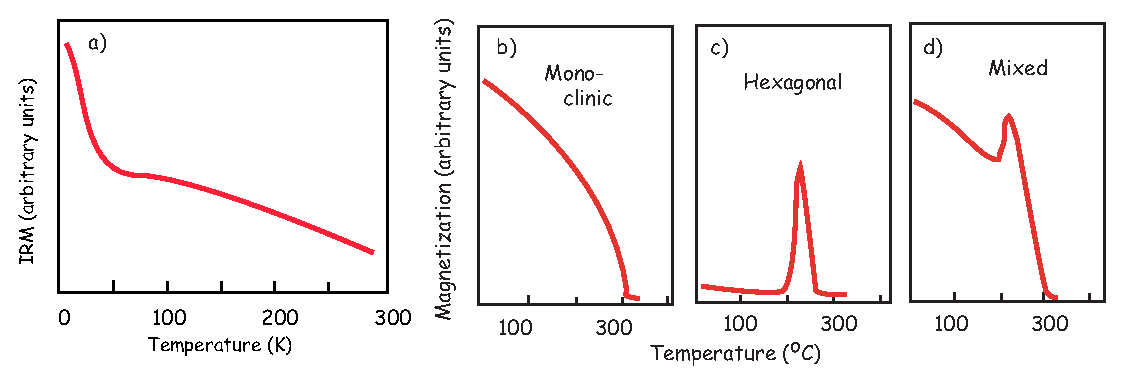
\includegraphics[width=13 cm]{EPSfiles/pyrrhotiteT.eps}
\caption{a) Low-temperature transition in monoclinic pyrhotite. [Data from Snowball and Torrii, 1999.]
 Thermomagnetic curves for b) monoclinic c) hexagonal and d) mixture of b) and c) pyrrhotite.  [Data from Dekkers, 1988.]}
\label{fig:pyrrhotiteT}
\end{figure}
\nocite{dekkers88}


\nocite{snowball99}





\section{FeTi oxides in igneous rocks}

The composition and relative proportions of FeTi oxides, crystallizing from a silicate melt depend on a number of factors, including the bulk chemistry of the melt, oxygen fugacity and the cooling rate. The final assemblage may be altered after cooling.  FeTi oxides are generally more abundant in mafic volcanic rocks (e.g. basalts) than silicic lavas (e.g., rhyolites).  FeTi oxides can be among the first liquidus phases ($\sim$ 1000$^{\circ}$C) in silicic melts, but in mafic lavas they generally are among the last phases to form ($\sim$1050$^{\circ}$C), often with plagioclase and pyroxene.  

Although there is considerable variability, the Ti (ulv\"ospinel) content of the titanomagnetite crystallizing from a melt generally is lower in more silicic melts (see solid black lines in Figure~\ref{fig:igneous}).   Titanomagnetites in tholeiitic lavas generally have 0.5 $<x<$ 0.8 with an initial composition near TM60 ($x$=0.6) characteristic for much of the oceanic crust.  The range of rhombohedral phases (dashed red lines)  crystallizing from silicate melts is more limited, $0.05<y<0.3$ for most lavas.   




\begin{figure}[htb]
%\centering \epsffile{EPSfiles/igneous.eps}
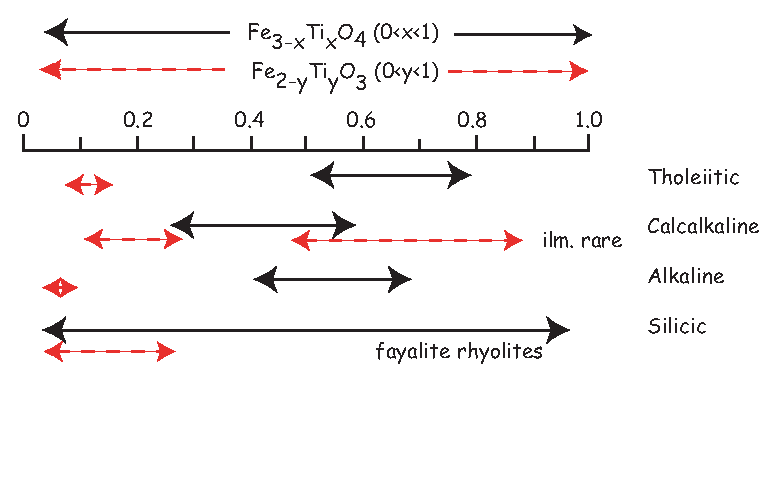
\includegraphics[width=13 cm]{EPSfiles/igneous.eps}
\caption{Occurrence of FeTi oxides in igneous rocks.  [Data from Frost and Lindsley, 1991.]}
\label{fig:igneous}
\end{figure}\nocite{frost91}


The final magnetic mineral assemblage in a rock is often strongly influenced by the cooling rate and oxygen fugacity during initial crystallization.  As a first approximation, we distinguish slowly cooled rocks (which may undergo solid state exsolution and/or deuteric oxidation) from those in which the oxide minerals were rapidly quenched.  As mentioned before, FeTi oxides in slowly cooled igneous rocks can exhibit exolution lamellae with bands of low and high titanium magnetites if the oxygen fugacity remains unoxidizing.   This reaction is very slow, so its effects are rarely seen in nature. 

The typical case in slowly cooled rocks is that the system becomes more oxidizing with increasing differentiation during cooling and crystallization.  For example, both the dissociation of magmatic water and the crystallization of silicate phases rich in Fe will act to increase the oxidation state.  This will drive compositions to higher $z$ values (see Figure~\ref{fig:tern}).  The final assemblage typically consists of ilmenite lamellae and a nearly pure magnetite host because adding $O_2$ drives the reaction 
$
Fe_2TiO_4 + O_2 \rightleftharpoons Fe_3O_4$
to the right.  This process is known as {\it oxyexsolution}.  Under even more oxidizing conditions, these phases may ultimately be replaced by their more oxidized counterparts (e.g., hematite, pseudobrookite).  

Weathering at ambient surface conditions or mild hydrothermal alteration may lead to the development of cation deficient (titano)maghemites.  This can either occur by addition of oxygen to the spinel phase with a corresponding oxidation of the Fe$^{2+}$ to Fe$^{3+}$ to maintain charge balance, or by the removal of some of the octahedral iron from the crystal structure.  


\begin{figure}[htb]
%\epsfxsize 14cm
%\centering \epsffile{EPSfiles/bacteria.eps}
\includegraphics[width=13 cm]{EPSfiles/bacteria.eps}
\caption{Photomicrographs of bacterial magnetites produced by magnetotactic bacteria.  a) Intact magnetosome in living bacterium. [False color image from H. Vali in Maher and Thompson, 1999.]  b) Chains recovered from ODP Site 1006D in the Bahamas [From M. Hounslow in Maher and Thompson, 1999.]}
\label{fig:bacteria}
\end{figure}
\nocite{maher99}
%\nocite{fassbinder90}



\section{Magnetic mineralogy of soils and sediments}

Igneous (and metamorphic) rocks are the ultimate source for the components of sedimentary rocks, but biological and low-temperature diagenetic agents work to modify these components and have a significant effect on magnetic mineralogy in sediments.  As a result there is a virtual rainbow of magnetic mineralogies found in sediments.     (Titano)magnetite coming into the sedimentary environment from an igneous source may experience a change in pH and redox conditions that make it no longer the stable phase, hence it may alter.   
Also,   although the geochemistry of seawater is generally oxidizing with respect to the stability field of magnetite, pronounced changes in the redox state of sediments often occur with increasing depth as a function of the breakdown of organic carbon.  Such changes may result in locally strongly reducing environments where magnetite may be dissolved and authigenic sulfides produced.  Indeed,  changes down sediment cores  in the ferrimagnetic mineral content and porewater geochemistry suggest that this process is active in some (most?) marine sedimentary sequences. For example, dissolution of magnetite and/or production of non-magnetic sulfides may be responsible for the oft-seen decrease in various bulk magnetic parameters (e.g., magnetic susceptibility, IRM, ARM, etc.) with depth.   




Some of the more spectacular magnetic minerals found in sediments are biogenic magnetites produced by magnetotactic bacteria (see recent review by Kopp and Kirsch- vink, 2008 and Figure~\ref{fig:bacteria}).   The sizes and shapes of
\index{magnetite!bacterial}
 bacterial magnetite, when plotted on the 
\index{diagrams!Evans}
 Evans diagram from Chapter 4, suggest that magnetotactic bacteria form magnetite in the single domain grain size range -- otherwise extremely rare in nature.    It appears that  bacterial magnetites are common in sediments, but their role in contributing to the  natural remanence is still poorly understood. 



 \nocite{oreilly84,dunlop97}
 \nocite{snowball90}\nocite{dekkers88}\nocite{dekkers89}\nocite{dekkers89b} \nocite{ozdemir93}\nocite{banerjee71}\nocite{worm93}\nocite{collinson83}\nocite{rochette90}\nocite{spender72}\nocite{snowball90}\nocite{roberts95}
\nocite{dunlop97}\nocite{dekkers89c}
 \begin{center}
\begin{longtable}{ll}
\caption [Physical properties of magnetic minerals.] {Physical properties of magnetic minerals.}
\label{tab:rockpars}\\

\hline
{Magnetite:}&Fe$_3$O$_4$\\
\endfirsthead

\multicolumn{2}{l}%
{\tablename\ \it  -- continued from previous page} \\
\hline
\endhead

\hline \multicolumn{2}{r}{{\it Continued on next page --}} \\
\endfoot
\hline
\endlastfoot

Density = 5197 kg m$^{-3}$& Dunlop and \"Ozdemir [1997]\\
{Curie temperature}  = 580$^{\circ}$C & Dunlop and \"Ozdemir [1997]\\
{Saturation Magnetization}  = 92 Am$^2$kg$^{-1}$&O'Reilly [1984]\\
{Anisotropy Constant} = -2.6 {Jkg}$^{-1}$&  Dunlop and \"Ozdemir [1997]\\
{Volume susceptibility} = $\sim$ 1 SI& O'Reilly [1984]\\
 {Typical coercivities are 10's of mT}& O'Reilly [1984] \\
 Verwey transition: 110-120 K& \" Ozdemir and Dunlop [1993]\\
Cell edge = 0.8396 nm & Dunlop and \"Ozdemir [1997]\\
\hline
Maghemite:&$\gamma$Fe$_2$O$_3$\\
Density = 5074 kg m$^{-3}$& Dunlop and \"Ozdemir [1997]\\
{Curie temperature}  = 590-675$^{\circ}$C & Dunlop and \"Ozdemir [1997]\\
{Saturation Magnetization}  = 74 Am$^2$kg$^{-1}$& Dunlop and \"Ozdemir
[1997]\\
{Anisotropy Constant} = 0.92 {Jkg}$^{-1}$&  Dunlop and \"Ozdemir [1997]\\
 Verwey transition: suppressed& Dunlop and \"Ozdemir [1997]\\ 
Breaks down to $\alpha$Fe$_2$O$_3$: between 250$\rightarrow$ 
750$^{\circ}$C &
Dunlop and \"Ozdemir [1997]\\
\hline
TM60:&Fe$_{2.4}$Ti$_{0.6}$O$_4$\\
Density = 4939 kg m$^{-3}$& Dunlop and \"Ozdemir [1997]\\
{Curie temperature}  = 150$^{\circ}$C & Dunlop and \"Ozdemir [1997]\\
{Saturation Magnetization}  = 24 Am$^2$kg$^{-1}$& Dunlop and \"Ozdemir
[1997]\\
{Anisotropy Constant} = 0.41 {Jkg}$^{-1}$&  Dunlop and \"Ozdemir [1997]\\
 {Coercivity $\sim$ 8 mT}& Dunlop and \"Ozdemir [1997]\\
Verwey transition: suppressed&Dunlop and \"Ozdemir [1997]\\
Cell edge = 0.8482 nm &Dunlop and \"Ozdemir [1997]\\
\hline
{Hematite:}&$\alpha$Fe$_2$O$_3$\\
Density = 5271 kg m$^{-3}$& Dunlop and \"Ozdemir [1997]\\
{N\' eel temperature} = 675$^{\circ}$C&O'Reilly [1984]\\
{Saturation Magnetization} = 0.4 Am$^2$kg$^{-1}$&O'Reilly [1984]\\
{Anisotropy Constant }  = 228 {Jkg}$^{-1}$&Dunlop and \"Ozdemir [1997]\\
{Volume susceptibility} = $\sim$ 1.3 x 10$^{-3}$ SI& O'Reilly [1984]\\
 {Coercivities vary widely and can be 10's of teslas}& 
Banerjee [1971]\\
Morin Transition: $\sim$ 250-260 K (for $>$ 0.2 $\mu$m)&O'Reilly [1984]\\
{Goethite:} & $\alpha$FeOOH\\
Density = 4264 kg m$^{-3}$& Dunlop and \"Ozdemir [1997]\\
{N\' eel temperature}: 70 $\rightarrow$ 125$^{\circ}$C & O'Reilly [1984]\\
{Saturation Magnetization} = 10$^{-3}\rightarrow$ 1 Am$^2$kg$^{-1}$ & O'Reilly [1984]\\
{Anisotropy Constant}  = 0.25 $\rightarrow $ 2 {Jkg}$^{-1}$&Dekkers [1989]\\
{Volume susceptibility} = $\sim$ 1 x 10$^{-3}$ SI& Dekkers [1989a]\\
 {Coercivities can be 10's of teslas}\\
Breaks down to hematite: 250 $\rightarrow$ 400$^{\circ}$C\\
\hline
{Pyrrhotite:} &Fe$_7$S$_8$\\
Density = 4662 kg m$^{-3}$& Dunlop and \"Ozdemir [1997]\\
Monoclinic:\\
{Curie temperature } = $\sim$ 325$^{\circ}$C&Dekkers [1989]\\
Hexagonal:\\
{Curie temperature } = $\sim$270$^{\circ}$C&Dekkers [1988]\\
{Saturation Magnetization} = 0.4 -$\sim$ 20 Am$^2$kg$^{-1}$&Worm et al. [1993]\\
{Volume susceptibility} = $\sim$ 1 x 10$^{-3}\rightarrow 1$ SI& Collinson [1983];O'Reilly [1984]\\
{Anisotropy Constant}  = 20 {Jkg}$^{-1}$&O'Reilly [1984]\\
 {Coercivities vary widely and can be 100's of mT}&O'Reilly [1984]\\
Has a transition at $\sim$ 34  K &Dekkers et al. [1989]\\
&Rochette et al. [1990] \\
Hexagonal pyrrotite:  transition near 200$^{\circ}$\\
Breaks down to magnetite: $\sim$ 500$^{\circ}$C&Dunlop and \"Ozdemir
[1997]\\
\hline
{Greigite:}&Fe$_3$S$_4$\\
Density = 4079 kg m$^{-3}$& Dunlop and \"Ozdemir [1997]\\
Maximum unblocking temperature = $\sim$ 330$^{\circ}$C&Roberts [1995]\\
{Saturation Magnetization} = $\sim$ 25 Am$^2$kg$^{-1}$&Spender et al. [1972]\\
{Anisotropy Constant}  = -0.25 {Jkg}$^{-1}$&Dunlop and \"Ozdemir
[1997]\\
{Coercivity 60$\rightarrow >$ 100 mT}& Roberts [1995]\\
Has high $M_r/\chi$ ratios $\sim$ 70 x 10$^3$ Am$^{-1}$& Snowball and Thompson
[1990]\\ 
{Breaks down to magnetite:}
 $\sim$ 270-350$^{\circ}$C&Roberts [1995]\\
\end{longtable}
\end{center}

\noindent{SUPPLEMENTAL READINGS:} Dunlop and \"Ozdemir (1997), Chapter 3;  
 Kopp and Kirschvink (2008). \nocite{kopp08}


\begin{figure}[htb]
%\epsfxsize 3in
%\centering \epsffile{EPSfiles/problem1.eps}
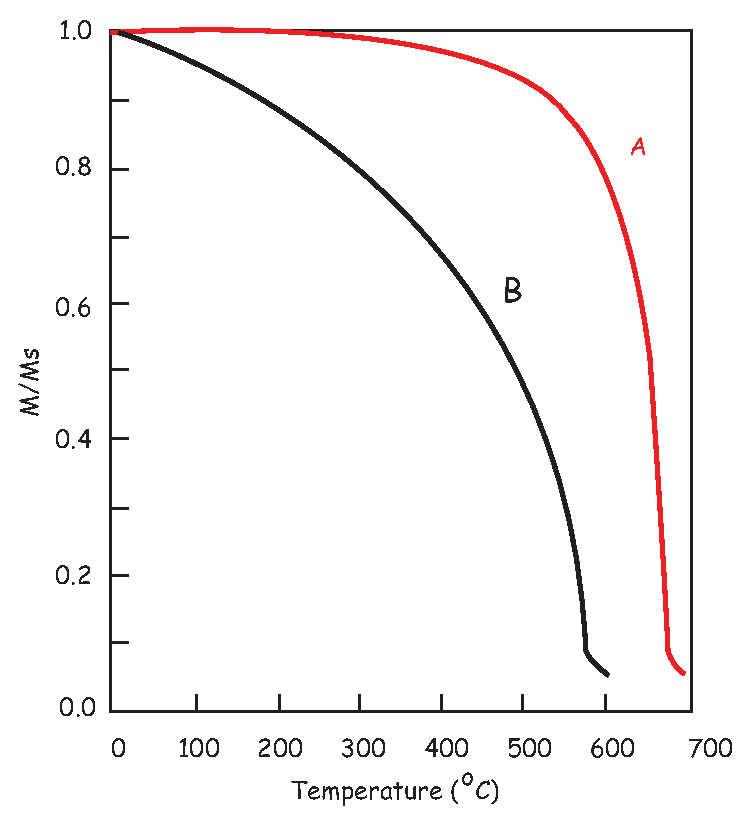
\includegraphics[width=3 cm]{EPSfiles/problem1.eps}
\caption{Curie Temperature curves for two samples, A and B. [Figure redrawn from Butler, 1992.]}
\label{fig:prob1}
\end{figure}

\clearpage

\nocite{butler92}
\section{Problems}




{{\parindent 0pt \parskip 12pt 

{\bf Problem 1}

You measured Curie Temperature curves for two samples A and B as shown in Figure~\ref{fig:prob1}.  Based on your knowledge of Curie Temperatures,  what is the likely magnetic mineralogy for each sample?  



{\bf Problem 2}

The data in {\it demag.dat} in the Chapter\_6 data directory (see Problems for  Chapter 5 for downloading instructions) are thermal demagnetization data for a 
specimen that had a 2 T field exposed along $x$, a 0.4 T field
exposed along $y$ and a 0.12 T field exposed along $z$.    The sample was then heated to a particular temperature
step ($^{\circ}$C) and cooled in zero magnetic field, allowing all grains that become superparamagnetic at temperatures lower than the treatment temperature to become randomized.  After each treatment step, the magnetic vector was measured.    The column headings are:  Treatment temperature (C), Intensity, Declination, Inclination.  


a) Write a python program to read the data in and convert the declination, inclination and intensity to cartesian components.  

b) Modify your program to normalize the intensity to the 20$^{\circ}$C  measurement. 

c)  Extend the program to plot  the $x$ and $y$ components as a function of temperature.   

d)  Based on your understanding of coercivity and Curie temperatures, what is carrying the $x$ and $y$ components?  

\begin{figure}[h!tb]
%\epsfxsize 12cm
%\centering \epsffile{EPSfiles/microprobe.eps}
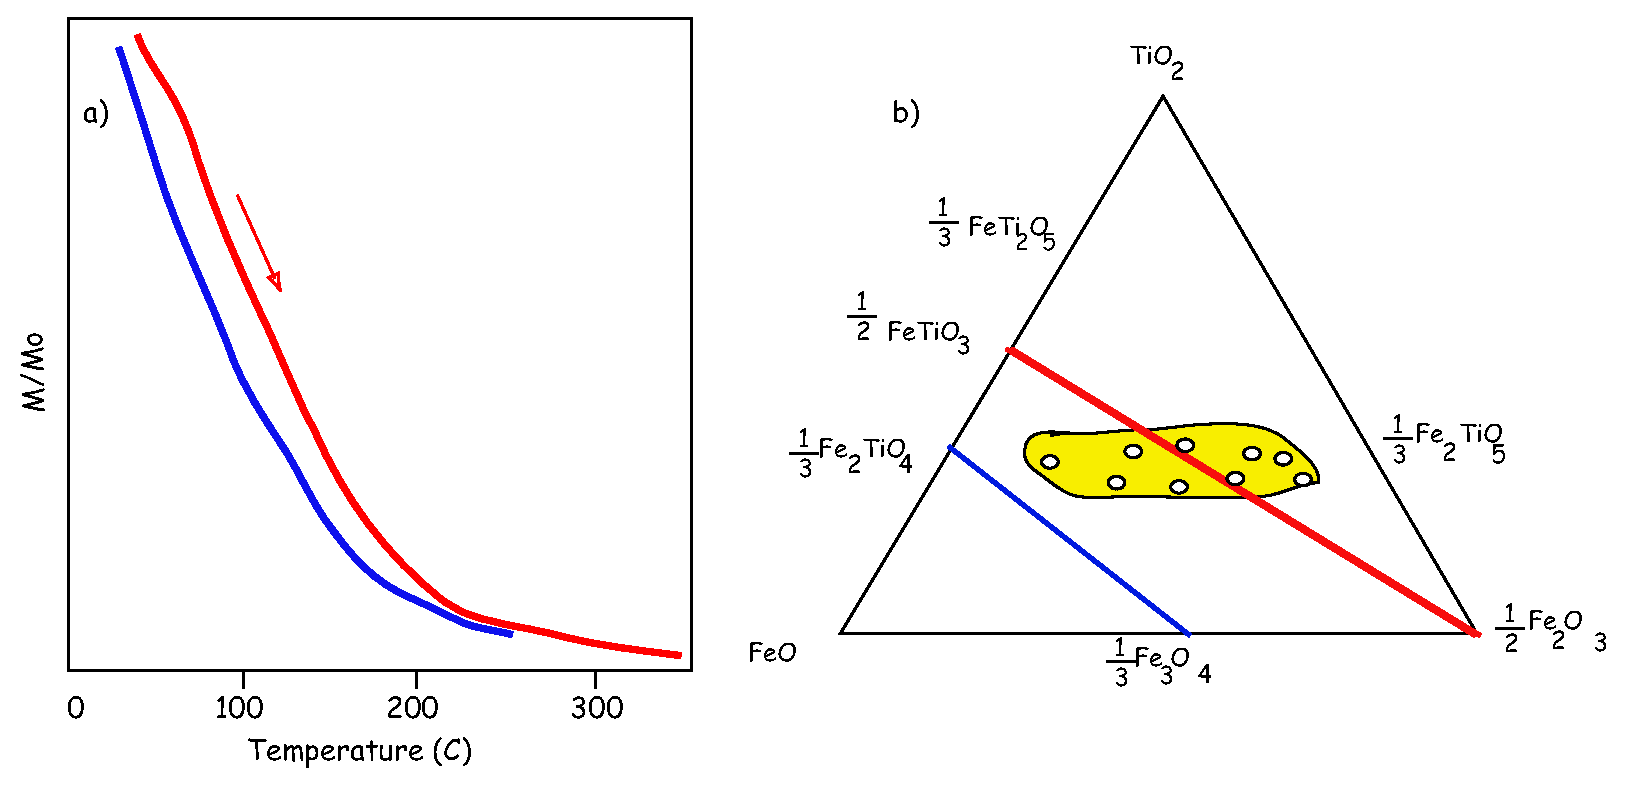
\includegraphics[width=13 cm]{EPSfiles/microprobe.eps}
\caption{a) Thermomagnetic run of mineral whereby magnetization (normalized by the initial value) is measured as a function of temperature.  The red line is the heating curve and the blue line is the cooling curve.  b) Electron microprobe data  from FeTi oxides (dots in yellow field) plotted on TiO$_2$-FeO-Fe$_2$O$_3$.
ternary diagram. [Figure redrawn from Butler, 1992.]}
\label{fig:microprobe}
\end{figure}



{\bf Problem 3}

Ferromagnetic minerals in two rock samples are known to be FeTi oxides and are found to have the
properties described below. Using this information and looking up the properties of FeTi oxides described
in the text, identify the ferromagnetic minerals. For titanomagnetite or titanohematite,
approximate the compositional parameter $x.$

a.) Strong-field thermomagnetic analysis indicates a dominant Curie temperature $T_c = 420^{\circ}$C. Subjecting the specimen to increasingly larger fields to measure successive isothermal remanences (see Chapter 5) 
reveals a coercivity spectrum with a coercivity of less than 300 mT. What is this ferromagnetic mineral?

b) Strong-field thermomagnetic analysis (used for measuring the Curie temperature)  shows the behavior in Figure~\ref{fig:microprobe}a  with Curie
temperature $T_c$ = 200$^{\circ}$C. In addition, electron microprobe data indicates abundances of FeO,
Fe$_2$O$_3$, and TiO shown in Figure~\ref{fig:microprobe}b. Unfortunately, electron microprobe data are not very
effective in determining the Fe$_2$O$_3$:FeO ratio (placement from left to right in the TiO-FeO-Fe$_2$O$_3$
ternary diagram). Accordingly, there is much uncertainty in the Fe$_2$O$_3$:FeO ratio indicated by
the microprobe data. But microprobe data are effective in determining the TiO:(Fe$_2$O$_3$ + FeO)
ratio (placement from bottom to top in the TiO-FeO-Fe$_2$O$_3$ ternary diagram). With this information,
identify the ferromagnetic mineral.



}

